\documentclass{standalone}
\usepackage{tikz}
\usetikzlibrary{patterns, positioning}
\usepackage[sfdefault]{ClearSans} %% option 'sfdefault' activates Clear Sans as the default text font
\usepackage[T1]{fontenc}

\begin{document}
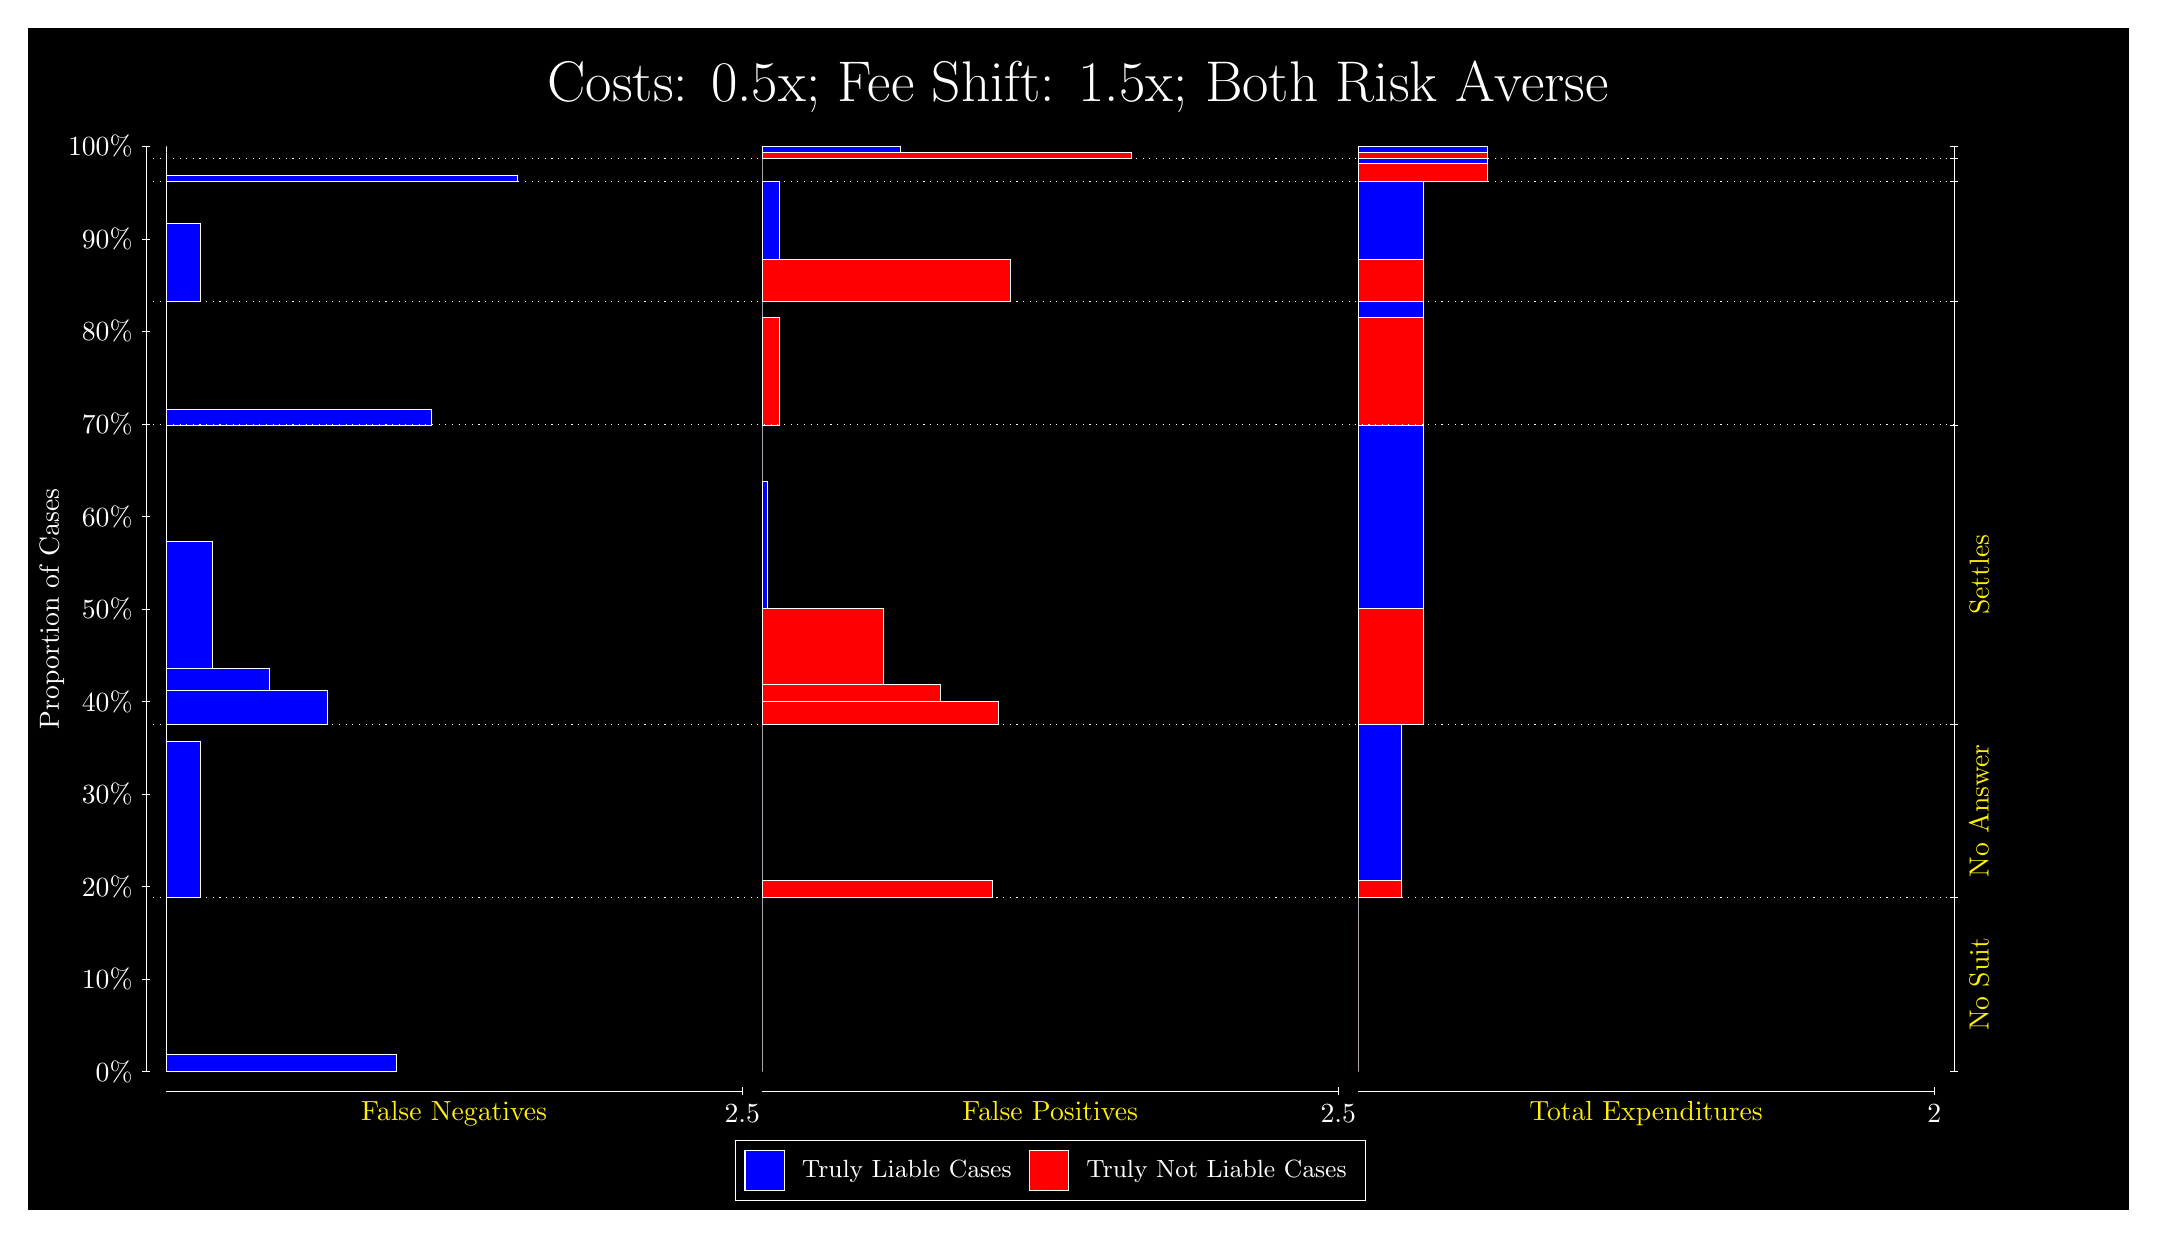
\begin{tikzpicture}
\draw[fill=black] (0,0) rectangle (26.667,15);
\draw[text=white] (0,13.5) rectangle (26.667,15) node[midway] {\huge Costs: 0.5x; Fee Shift: 1.5x; Both Risk Averse};
\draw[white, very thin] (1.5,1.75) -- (1.5,13.5);
\node[rotate=90, text=white, anchor=center] at (0.3, 7.625) {Proportion of Cases};
\draw[white, very thin] (1.45,1.75) -- (1.55,1.75);
\node[text=white, anchor=east] at (1.45, 1.75) {0\%};
\draw[white, very thin] (1.45,2.925) -- (1.55,2.925);
\node[text=white, anchor=east] at (1.45, 2.925) {10\%};
\draw[white, very thin] (1.45,4.1) -- (1.55,4.1);
\node[text=white, anchor=east] at (1.45, 4.1) {20\%};
\draw[white, very thin] (1.45,5.275) -- (1.55,5.275);
\node[text=white, anchor=east] at (1.45, 5.275) {30\%};
\draw[white, very thin] (1.45,6.45) -- (1.55,6.45);
\node[text=white, anchor=east] at (1.45, 6.45) {40\%};
\draw[white, very thin] (1.45,7.625) -- (1.55,7.625);
\node[text=white, anchor=east] at (1.45, 7.625) {50\%};
\draw[white, very thin] (1.45,8.8) -- (1.55,8.8);
\node[text=white, anchor=east] at (1.45, 8.8) {60\%};
\draw[white, very thin] (1.45,9.975) -- (1.55,9.975);
\node[text=white, anchor=east] at (1.45, 9.975) {70\%};
\draw[white, very thin] (1.45,11.15) -- (1.55,11.15);
\node[text=white, anchor=east] at (1.45, 11.15) {80\%};
\draw[white, very thin] (1.45,12.325) -- (1.55,12.325);
\node[text=white, anchor=east] at (1.45, 12.325) {90\%};
\draw[white, very thin] (1.45,13.5) -- (1.55,13.5);
\node[text=white, anchor=east] at (1.45, 13.5) {100\%};

\draw[white, very thin] (24.457,1.75) -- (24.457,13.5);
\draw[white, very thin] (24.407,1.75) -- (24.507,1.75);
\node[anchor=west] at (24.407, 1.75) {};
\draw[white, very thin] (24.407,3.9624) -- (24.507,3.9624);
\node[anchor=west] at (24.407, 3.9624) {};
\draw[white, very thin] (24.407,6.159) -- (24.507,6.159);
\node[anchor=west] at (24.407, 6.159) {};
\draw[white, very thin] (24.407,9.9616) -- (24.507,9.9616);
\node[anchor=west] at (24.407, 9.9616) {};
\draw[white, very thin] (24.407,11.532) -- (24.507,11.532);
\node[anchor=west] at (24.407, 11.532) {};
\draw[white, very thin] (24.407,13.058) -- (24.507,13.058);
\node[anchor=west] at (24.407, 13.058) {};
\draw[white, very thin] (24.407,13.351) -- (24.507,13.351);
\node[anchor=west] at (24.407, 13.351) {};
\draw[white, very thin] (24.407,13.5) -- (24.507,13.5);
\node[anchor=west] at (24.407, 13.5) {};

\draw[white, very thin, fill=blue] (1.75,1.75) rectangle (4.6775,1.9721);
\draw[white, very thin, fill=red] (1.75,1.9721) rectangle (1.75,3.9624);
\draw[white, very thin, fill=blue] (1.75,3.9624) rectangle (2.1891,5.9447);
\draw[white, very thin, fill=red] (1.75,5.9447) rectangle (1.75,6.159);
\draw[white, very thin, fill=blue] (1.75,6.159) rectangle (3.7993,6.5967);
\draw[white, very thin, fill=blue] (1.75,6.5967) rectangle (3.0674,6.8688);
\draw[white, very thin, fill=blue] (1.75,6.8688) rectangle (2.3355,8.4829);
\draw[white, very thin, fill=red] (1.75,8.4829) rectangle (1.75,9.9616);
\draw[white, very thin, fill=blue] (1.75,9.9616) rectangle (5.1167,10.164);
\draw[white, very thin, fill=red] (1.75,10.164) rectangle (1.75,11.532);
\draw[white, very thin, fill=blue] (1.75,11.532) rectangle (2.1891,12.528);
\draw[white, very thin, fill=red] (1.75,12.528) rectangle (1.75,13.058);
\draw[white, very thin, fill=blue] (1.75,13.058) rectangle (6.2145,13.129);
\draw[white, very thin, fill=red] (1.75,13.129) rectangle (1.75,13.351);
\draw[white, very thin, fill=red] (1.75,13.351) rectangle (1.75,13.422);
\draw[white, very thin, fill=blue] (1.75,13.422) rectangle (1.75,13.5);
\draw[white, very thin, fill=red] (9.3189,1.75) rectangle (9.3189,3.7403);
\draw[white, very thin, fill=blue] (9.3189,3.7403) rectangle (9.3189,3.9624);
\draw[white, very thin, fill=red] (9.3189,3.9624) rectangle (12.246,4.1767);
\draw[white, very thin, fill=blue] (9.3189,4.1767) rectangle (9.3189,6.159);
\draw[white, very thin, fill=red] (9.3189,6.159) rectangle (12.32,6.4579);
\draw[white, very thin, fill=red] (9.3189,6.4579) rectangle (11.588,6.6662);
\draw[white, very thin, fill=red] (9.3189,6.6662) rectangle (10.856,7.6377);
\draw[white, very thin, fill=blue] (9.3189,7.6377) rectangle (9.3921,9.2518);
\draw[white, very thin, fill=blue] (9.3189,9.2518) rectangle (9.3189,9.9616);
\draw[white, very thin, fill=red] (9.3189,9.9616) rectangle (9.5384,11.33);
\draw[white, very thin, fill=blue] (9.3189,11.33) rectangle (9.3189,11.532);
\draw[white, very thin, fill=red] (9.3189,11.532) rectangle (12.466,12.063);
\draw[white, very thin, fill=blue] (9.3189,12.063) rectangle (9.5384,13.058);
\draw[white, very thin, fill=red] (9.3189,13.058) rectangle (9.3189,13.28);
\draw[white, very thin, fill=blue] (9.3189,13.28) rectangle (9.3189,13.351);
\draw[white, very thin, fill=red] (9.3189,13.351) rectangle (14.003,13.422);
\draw[white, very thin, fill=blue] (9.3189,13.422) rectangle (11.075,13.5);
\draw[white, very thin, fill=red] (16.888,1.75) rectangle (16.888,3.7403);
\draw[white, very thin, fill=blue] (16.888,3.7403) rectangle (16.888,3.9624);
\draw[white, very thin, fill=red] (16.888,3.9624) rectangle (17.437,4.1767);
\draw[white, very thin, fill=blue] (16.888,4.1767) rectangle (17.437,6.159);
\draw[white, very thin, fill=red] (16.888,6.159) rectangle (17.711,7.6377);
\draw[white, very thin, fill=blue] (16.888,7.6377) rectangle (17.711,9.9616);
\draw[white, very thin, fill=red] (16.888,9.9616) rectangle (17.711,11.33);
\draw[white, very thin, fill=blue] (16.888,11.33) rectangle (17.711,11.532);
\draw[white, very thin, fill=red] (16.888,11.532) rectangle (17.711,12.063);
\draw[white, very thin, fill=blue] (16.888,12.063) rectangle (17.711,13.058);
\draw[white, very thin, fill=red] (16.888,13.058) rectangle (18.534,13.28);
\draw[white, very thin, fill=blue] (16.888,13.28) rectangle (18.534,13.351);
\draw[white, very thin, fill=red] (16.888,13.351) rectangle (18.534,13.422);
\draw[white, very thin, fill=blue] (16.888,13.422) rectangle (18.534,13.5);
\draw[white, dotted] (1.5,3.9624) -- (24.457,3.9624);
\draw[white, dotted] (1.5,6.159) -- (24.457,6.159);
\draw[white, dotted] (1.5,9.9616) -- (24.457,9.9616);
\draw[white, dotted] (1.5,11.532) -- (24.457,11.532);
\draw[white, dotted] (1.5,13.058) -- (24.457,13.058);
\draw[white, dotted] (1.5,13.351) -- (24.457,13.351);
\draw[white, very thin] (1.75,1.5) -- (9.0689,1.5);
\node[text=yellow, anchor=north] at (5.4094, 1.5) {False Negatives};
\draw[white, very thin] (9.0689,1.45) -- (9.0689,1.55);
\node[text=white, anchor=north] at (9.0689, 1.45) {2.5};

\draw[white, very thin] (9.3189,1.5) -- (16.638,1.5);
\node[text=yellow, anchor=north] at (12.978, 1.5) {False Positives};
\draw[white, very thin] (16.638,1.45) -- (16.638,1.55);
\node[text=white, anchor=north] at (16.638, 1.45) {2.5};

\draw[white, very thin] (16.888,1.5) -- (24.207,1.5);
\node[text=yellow, anchor=north] at (20.547, 1.5) {Total Expenditures};
\draw[white, very thin] (24.207,1.45) -- (24.207,1.55);
\node[text=white, anchor=north] at (24.207, 1.45) {2};

\node[text=yellow, centered, rotate=90] at (24.777, 2.8562) {No Suit};
\node[text=yellow, centered, rotate=90] at (24.777, 5.0607) {No Answer};
\node[text=yellow, centered, rotate=90] at (24.777, 8.0603) {Settles};





\draw (12.978300999999998,1.5) node[draw=none] (baseCoordinate) {};
\begin{scope}[align=center]
        \matrix[scale=0.5, draw=white, below=0.5cm of baseCoordinate, nodes={draw}, column sep=0.1cm]{
            \node[rectangle, draw, minimum width=0.5cm, minimum height=0.5cm, fill=blue] {}; &
            \node[draw=none, font=\small, text=white] (B) {Truly Liable Cases}; &
            \node[rectangle, draw, minimum width=0.5cm, minimum height=0.5cm, fill=red] {}; &
            \node[draw=none, font=\small, text=white] (B) {Truly Not Liable Cases}; \\
            };
\end{scope}

\end{tikzpicture}
\end{document}